% !TeX program = XeLaTeX
% !TeX encoding = UTF-8

\documentclass[11pt]{report}

\usepackage{hyperref}
\hypersetup{
    colorlinks = true,
    allcolors = {red}
}
\usepackage{url}
\usepackage[bottom]{footmisc}
\usepackage{subcaption}

% \usepackage{CJKutf8} % For Japanese UTF-8 text in pdflatex

% For Japanese UTF-8 text in XeLaTeX
\usepackage{xeCJK}
\setCJKmainfont{IPAexMincho}


\usepackage[japanese]{babel} % For Japanese date format
\usepackage{indentfirst} % For Japanese style indentation
\setlength\parindent{11pt}

%%%%%%%%%%%%%%%%
% For the margins
\usepackage{geometry}
\geometry{
    paper=a4paper, inner=2.5cm, outer=2.5cm, bindingoffset=.5cm, top=1.5cm, bottom=1.5cm, }
%%%%%%%%%%%%%%%%

%%%%%%%%%
% For the affiliation command to work in \maketitle
\usepackage{etoolbox}
\makeatletter
\providecommand{\affiliation}[1]{% add affiliation to \maketitle
  \apptocmd{\@author}{\end{tabular}
    \par
    \begin{tabular}[t]{c}
    \small #1}{}{}
}
\makeatother
%%%%%%%%%

%%%%%%%%%
% For the projectnotes command to work in \maketitle
\usepackage{etoolbox}
\makeatletter
\providecommand{\projectnotes}[1]{% add projectnotes to \maketitle
  \apptocmd{\@author}{
    \end{tabular}
    \vspace{10em}
    \par
    \begin{tabular}[t]{l}
    \small #1 
    \vspace{10em}
    }{}{}
}
\makeatother
%%%%%%%%%

%%%%%%%%%%%%%%%%%%%%%%%%%%%%%%%%%%%%%%%%
%%%%%%%%%%%%%%%%%%%%%%%%%%%%%%%%%%%%%%%%
%%%%%%%%%%%%%%%%%%%%%%%%%%%%%%%%%%%%%%%%
\usepackage[lighttt]{lmodern}
\usepackage{listings} % to display code
\usepackage{lstautogobble} % to indent inside latex without affecting the code, keeping the indent the code has inside
\usepackage{anyfontsize} % for code font size
\usepackage[os=win]{menukeys} % to display keystrokes

% For the color behind the code sections:
\usepackage{xcolor} %custom colours
\definecolor{light-gray}{gray}{0.95} %the shade of grey that stack exchange uses
\definecolor{editorGreen}{rgb}{0, 0.5, 0} % #007C00 -> rgb(0, 124, 0)

% Make a more defined languages for nice colors
\lstdefinelanguage{CSS}{
      keywords={*,html,body,a,h1,h2,h3,h4,h5,h6,h7,h8,h9,p,form,button,label,input,textarea,select,table,th,td,tr,header,footer,and
      },
      morekeywords={[2]{-moz-binding, -moz-border-bottom-colors, -moz-border-left-colors, -moz-border-radius, -moz-border-radius-bottomleft, -moz-border-radius-bottomright, -moz-border-radius-topleft, -moz-border-radius-topright, -moz-border-right-colors, -moz-border-top-colors, -moz-opacity, -moz-outline, -moz-outline-color, -moz-outline-style, -moz-outline-width, -moz-user-focus, -moz-user-input, -moz-user-modify, -moz-user-select, -replace, -set-link-source, -use-link-source, accelerator, align-content, align-items, align-self, animation-delay, animation-direction, animation-duration, animation-fill-mode, animation-iteration-count, animation-name, animation-play-state, animation-timing-function, animation, azimuth, backface-visibility, background, background-attachment, background-clip, background-color, background-image, background-origin, background-position, background-position-x, background-position-y, background-repeat, background-size, behavior, border, border-bottom, border-bottom-color, border-bottom-left-radius, border-bottom-right-radius, border-bottom-style, border-bottom-width, border-collapse, border-color, border-image-outset, border-image-repeat, border-image-slice, border-image-source, border-image-width, border-image, border-left, border-left-color, border-left-style, border-left-width, border-radius, border-right, border-right-color, border-right-style, border-right-width, border-spacing, border-style, border-top, border-top-color, border-top-left-radius, border-top-right-radius, border-top-style, border-top-width, border-width, bottom, box-shadow, box-sizing, caption-side, clear, clip, color, column-count, column-fill, column-gap, column-rule-color, column-rule-style, column-rule-width, column-rule, column-span, column-width, columns, content, counter-increment, counter-reset, cue, cue-after, cue-before, cursor, direction, display, elevation, empty-cells, filter, flex-basis, flex-direction, flex-flow, flex-grow, flex-shrink, flex-wrap, flex, float, font, font-family, font-size, font-size-adjust, font-stretch, font-style, font-variant, font-weight, height, ime-mode, include-source, justify-content, layer-background-color, layer-background-image, layout-flow, layout-grid, layout-grid-char, layout-grid-char-spacing, layout-grid-line, layout-grid-mode, layout-grid-type, left, letter-spacing, line-break, line-height, list-style, list-style-image, list-style-position, list-style-type, margin, margin-bottom, margin-left, margin-right, margin-top, marker-offset, marks, max-height, max-width, min-height, min-width, opacity, order, orphans, outline, outline-color, outline-offset, outline-style, outline-width, overflow, overflow-wrap, overflow-X, overflow-x, overflow-Y, overflow-y, padding, padding-bottom, padding-left, padding-right, padding-top, page, page-break-after, page-break-before, page-break-inside, pause, pause-after, pause-before, perspective-origin, perspective, pitch, pitch-range, play-during, position, quotes, resize, richness, right, ruby-align, ruby-overhang, ruby-position, scrollbar-3d-light-color, scrollbar-arrow-color, scrollbar-base-color, scrollbar-dark-shadow-color, scrollbar-face-color, scrollbar-highlight-color, scrollbar-shadow-color, scrollbar-track-color, size, speak, speak-header, speak-numeral, speak-punctuation, speech-rate, stress, tab-size, table-layout, text-align, text-align-last, text-autospace, text-decoration, text-decoration-color, text-decoration-line, text-decoration-style, text-indent, text-justify, text-kashida-space, text-overflow, text-shadow, text-transform, text-underline-position, top, transform-origin, transform-style, transform, transition-delay, transition-duration, transition-property, transition-timing-function, transition, unicode-bidi, vertical-align, visibility, voice-family, volume, white-space, widows, width, word-break, word-spacing, word-wrap, writing-mode, z-index, zoom
        }}, 
      sensitive=true,
      morecomment=[l]{//},
      morecomment=[s]{/*}{*/},
      morestring=[b]',
      morestring=[b]",
      alsoother={:},
      alsodigit={-},
      tag=[s]
    }
\lstdefinelanguage{HTML5}{
            language=html,
            sensitive=true, 
            alsoletter={<>=-},
            otherkeywords={
            % HTML tags
            <, </, >,
            </a, <a, </a>,
            </abbr, <abbr, </abbr>,
            </address, <address, </address>,
            </area, <area, </area>,
            </area, <area, </area>,
            </article, <article, </article>,
            </aside, <aside, </aside>,
            </audio, <audio, </audio>,
            </audio, <audio, </audio>,
            </b, <b, </b>,
            </base, <base, </base>,
            </bdi, <bdi, </bdi>,
            </bdo, <bdo, </bdo>,
            </blockquote, <blockquote, </blockquote>,
            </body, <body, </body>,
            </br, <br, </br>,
            </button, <button, </button>,
            </canvas, <canvas, </canvas>,
            </caption, <caption, </caption>,
            </cite, <cite, </cite>,
            </code, <code, </code>,
            </col, <col, </col>,
            </colgroup, <colgroup, </colgroup>,
            </data, <data, </data>,
            </datalist, <datalist, </datalist>,
            </dd, <dd, </dd>,
            </del, <del, </del>,
            </details, <details, </details>,
            </dfn, <dfn, </dfn>,
            </div, <div, </div>,
            </dl, <dl, </dl>,
            </dt, <dt, </dt>,
            </em, <em, </em>,
            </embed, <embed, </embed>,
            </fieldset, <fieldset, </fieldset>,
            </figcaption, <figcaption, </figcaption>,
            </figure, <figure, </figure>,
            </footer, <footer, </footer>,
            </form, <form, </form>,
            </h1, <h1, </h1>,
            </h2, <h2, </h2>,
            </h3, <h3, </h3>,
            </h4, <h4, </h4>,
            </h5, <h5, </h5>,
            </h6, <h6, </h6>,
            </head, <head, </head>,
            </header, <header, </header>,
            </hr, <hr, </hr>,
            </html, <html, </html>,
            </i, <i, </i>,
            </iframe, <iframe, </iframe>,
            </img, <img, </img>,
            </input, <input, </input>,
            </ins, <ins, </ins>,
            </kbd, <kbd, </kbd>,
            </keygen, <keygen, </keygen>,
            </label, <label, </label>,
            </legend, <legend, </legend>,
            </li, <li, </li>,
            </link, <link, </link>,
            </main, <main, </main>,
            </map, <map, </map>,
            </mark, <mark, </mark>,
            </math, <math, </math>,
            </menu, <menu, </menu>,
            </menuitem, <menuitem, </menuitem>,
            </meta, <meta, </meta>,
            </meter, <meter, </meter>,
            </nav, <nav, </nav>,
            </noscript, <noscript, </noscript>,
            </object, <object, </object>,
            </ol, <ol, </ol>,
            </optgroup, <optgroup, </optgroup>,
            </option, <option, </option>,
            </output, <output, </output>,
            </p, <p, </p>,
            </param, <param, </param>,
            </pre, <pre, </pre>,
            </progress, <progress, </progress>,
            </q, <q, </q>,
            </rp, <rp, </rp>,
            </rt, <rt, </rt>,
            </ruby, <ruby, </ruby>,
            </s, <s, </s>,
            </samp, <samp, </samp>,
            </script, <script, </script>,
            </section, <section, </section>,
            </select, <select, </select>,
            </small, <small, </small>,
            </source, <source, </source>,
            </span, <span, </span>,
            </strong, <strong, </strong>,
            </style, <style, </style>,
            </summary, <summary, </summary>,
            </sup, <sup, </sup>,
            </svg, <svg, </svg>,
            </table, <table, </table>,
            </tbody, <tbody, </tbody>,
            </td, <td, </td>,
            </template, <template, </template>,
            </textarea, <textarea, </textarea>,
            </tfoot, <tfoot, </tfoot>,
            </th, <th, </th>,
            </thead, <thead, </thead>,
            </time, <time, </time>,
            </title, <title, </title>,
            </tr, <tr, </tr>,
            </track, <track, </track>,
            </u, <u, </u>,
            </ul, <ul, </ul>,
            </var, <var, </var>,
            </video, <video, </video>,
            </wbr, <wbr, </wbr>,
            />, <!
            },  
            morekeywords={[2]{
            % General
            =,
            % HTML attributes
            accept=, accept-charset=, accesskey=, action=, align=, alt=, async=, autocomplete=, autofocus=, autoplay=, autosave=, bgcolor=, border=, buffered=, challenge=, charset=, checked=, cite=, class=, code=, codebase=, color=, cols=, colspan=, content=, contenteditable=, contextmenu=, controls=, coords=, data=, datetime=, default=, defer=, dir=, dirname=, disabled=, download=, draggable=, dropzone=, enctype=, for=, form=, formaction=, headers=, height=, hidden=, high=, href=, hreflang=, http-equiv=, icon=, id=, ismap=, itemprop=, keytype=, kind=, label=, lang=, language=, list=, loop=, low=, manifest=, max=, maxlength=, media=, method=, min=, multiple=, name=, novalidate=, open=, optimum=, pattern=, ping=, placeholder=, poster=, preload=, pubdate=, radiogroup=, readonly=, rel=, required=, reversed=, rows=, rowspan=, sandbox=, scope=, scoped=, seamless=, selected=, shape=, size=, sizes=, span=, spellcheck=, src=, srcdoc=, srclang=, start=, step=, style=, summary=, tabindex=, target=, title=, type=, usemap=, value=, width=, wrap=,
            % CSS properties
            -moz-binding:, -moz-border-bottom-colors:, -moz-border-left-colors:, -moz-border-radius:, -moz-border-radius-bottomleft:, -moz-border-radius-bottomright:, -moz-border-radius-topleft:, -moz-border-radius-topright:, -moz-border-right-colors:, -moz-border-top-colors:, -moz-opacity:, -moz-outline:, -moz-outline-color:, -moz-outline-style:, -moz-outline-width:, -moz-user-focus:, -moz-user-input:, -moz-user-modify:, -moz-user-select:, -replace:, -set-link-source:, -use-link-source:, accelerator:, align-content:, align-items:, align-self:, animation-delay:, animation-direction:, animation-duration:, animation-fill-mode:, animation-iteration-count:, animation-name:, animation-play-state:, animation-timing-function:, animation:, azimuth:, backface-visibility:, background:, background-attachment:, background-clip:, background-color:, background-image:, background-origin:, background-position:, background-position-x:, background-position-y:, background-repeat:, background-size:, behavior:, border:, border-bottom:, border-bottom-color:, border-bottom-left-radius:, border-bottom-right-radius:, border-bottom-style:, border-bottom-width:, border-collapse:, border-color:, border-image-outset:, border-image-repeat:, border-image-slice:, border-image-source:, border-image-width:, border-image:, border-left:, border-left-color:, border-left-style:, border-left-width:, border-radius:, border-right:, border-right-color:, border-right-style:, border-right-width:, border-spacing:, border-style:, border-top:, border-top-color:, border-top-left-radius:, border-top-right-radius:, border-top-style:, border-top-width:, border-width:, bottom:, box-shadow:, box-sizing:, caption-side:, clear:, clip:, color:, column-count:, column-fill:, column-gap:, column-rule-color:, column-rule-style:, column-rule-width:, column-rule:, column-span:, column-width:, columns:, content:, counter-increment:, counter-reset:, cue:, cue-after:, cue-before:, cursor:, direction:, display:, elevation:, empty-cells:, filter:, flex-basis:, flex-direction:, flex-flow:, flex-grow:, flex-shrink:, flex-wrap:, flex:, float:, font:, font-family:, font-size:, font-size-adjust:, font-stretch:, font-style:, font-variant:, font-weight:, height:, ime-mode:, include-source:, justify-content:, layer-background-color:, layer-background-image:, layout-flow:, layout-grid:, layout-grid-char:, layout-grid-char-spacing:, layout-grid-line:, layout-grid-mode:, layout-grid-type:, left:, letter-spacing:, line-break:, line-height:, list-style:, list-style-image:, list-style-position:, list-style-type:, margin:, margin-bottom:, margin-left:, margin-right:, margin-top:, marker-offset:, marks:, max-height:, max-width:, min-height:, min-width:, opacity:, order:, orphans:, outline:, outline-color:, outline-offset:, outline-style:, outline-width:, overflow:, overflow-wrap:, overflow-X:, overflow-x:, overflow-Y:, overflow-y:, padding:, padding-bottom:, padding-left:, padding-right:, padding-top:, page:, page-break-after:, page-break-before:, page-break-inside:, pause:, pause-after:, pause-before:, perspective-origin:, perspective:, pitch:, pitch-range:, play-during:, position:, quotes:, resize:, richness:, right:, ruby-align:, ruby-overhang:, ruby-position:, scrollbar-3d-light-color:, scrollbar-arrow-color:, scrollbar-base-color:, scrollbar-dark-shadow-color:, scrollbar-face-color:, scrollbar-highlight-color:, scrollbar-shadow-color:, scrollbar-track-color:, size:, speak:, speak-header:, speak-numeral:, speak-punctuation:, speech-rate:, stress:, tab-size:, table-layout:, text-align:, text-align-last:, text-autospace:, text-decoration:, text-decoration-color:, text-decoration-line:, text-decoration-style:, text-indent:, text-justify:, text-kashida-space:, text-overflow:, text-shadow:, text-transform:, text-underline-position:, top:, transform-origin:, transform-style:, transform:, transition-delay:, transition-duration:, transition-property:, transition-timing-function:, transition:, unicode-bidi:, vertical-align:, visibility:, voice-family:, volume:, white-space:, widows:, width:, word-break:, word-spacing:, word-wrap:, writing-mode:, z-index:, zoom:
            }},  
            morecomment=[s]{<!--}{-->},
            tag=[s]
    }

% Set up the code display lst options
\lstset{
    % for the code font and size:
    % basicstyle=\ttfamily\small,
    basicstyle=\ttfamily\fontsize{10}{12}\selectfont,
    % to avoid spaces showing as brackets in strings
    showstringspaces=false,
    % for straight quotes in code
    upquote=true, 
    % for the middle tildes in the code
    literate={~}{{\fontfamily{ptm}\selectfont \textasciitilde}}1,
    % for the line break in long texts
    breaklines=true,
    postbreak=\mbox{\textcolor{red}{$\hookrightarrow$}\space}, 
    % for the keyword colors in the code
    keywordstyle=\color{blue}\bfseries\ttfamily,
    stringstyle=\color{purple},
    commentstyle=\color{darkgray}\ttfamily,
    keywordstyle={[2]{\color{editorGreen}\bfseries\ttfamily}},
    autogobble=true % to ignore latex indents but keep code indent
}

% unnecessary in XeLaTeX
% % For this specific document with lots of degree signs inside listings
% \lstset{
%     literate={°}{\textdegree}1
% }

% for straight double quotes in code
\usepackage[T1]{fontenc}

% frame set up
\usepackage[framemethod=TikZ]{mdframed} %nice frames
\mdfsetup{
    backgroundcolor=light-gray,
    roundcorner=7pt,
    leftmargin=1,
    rightmargin=1,
    innerleftmargin=1em,
    innertopmargin=0.5em,
    innerbottommargin=0,
    outerlinewidth=1,
    linecolor=light-gray,
    } 

% Make it affect all lstlistings
\BeforeBeginEnvironment{lstlisting}{\begin{mdframed}\vskip-.5\baselineskip}
\AfterEndEnvironment{lstlisting}{\end{mdframed}}

% Make colored box around inline code
\usepackage{realboxes}
\usepackage{xpatch}

\makeatletter
\xpretocmd\lstinline{\Colorbox{light-gray}\bgroup\appto\lst@DeInit{\egroup}}{}{}
\makeatother

%%%%%%%%%%%%%%%%%%%%%%%%%%%%%%%%%%%%%%%%
%%%%%%%%%%%%%%%%%%%%%%%%%%%%%%%%%%%%%%%%
%%%%%%%%%%%%%%%%%%%%%%%%%%%%%%%%%%%%%%%%

%%%%%%%%%%%%%%%%%%%%%%
% To make numbered paragraphs
\usepackage{titlesec}

\setcounter{secnumdepth}{4} 
% For deeper numbered sections

\titleformat{\paragraph}
{\normalfont\normalsize\bfseries}{\theparagraph}{0.2em}{} % space after number
\titlespacing*{\paragraph}
{1.2em}{1em}{1em} %left indent, upper and lower spacing (same as an enumerate)


\renewcommand\theparagraph{\arabic{paragraph}.}

% \usepackage{enumitem} % For nested enumerates to have numbers
%%%%%%%%%%%%%%%%%%%%%%

\usepackage{nameref} % To reference sections by name

%bibliography
\usepackage[
    backend=bibtex
    ,style=numeric
    ,natbib=true
    ,sorting=none
    ,url=true
    ,doi=true
    ]{biblatex}
\renewbibmacro*{urldate}{
    (アクセス日: \printfield{urlyear}年\printfield{urlmonth}月\printfield{urlday}日)
}
\addbibresource{report.bib}


%%%%%%%%%%%%%%%%%%%%%%%%%%%%%%%%%%%%%%%%%%%%%%
%%%%%%%%%%%%%%%%%%%%%%%%%%%%%%%%%%%%%%%%%%%%%%
%%%%%%%%%%%%%%%%%%%%%%%%%%%%%%%%%%%%%%%%%%%%%%
%%%%%%%%%%%%%%%%%%%%%%%%%%%%%%%%%%%%%%%%%%%%%%
%%%%%%%%%%%%%%%%%%%%%%%%%%%%%%%%%%%%%%%%%%%%%%
%%%%%%%%%%%%%%%%%%%%%%%%%%%%%%%%%%%%%%%%%%%%%%
%%%%%%%%%%%%%%%%%%%%%%%%%%%%%%%%%%%%%%%%%%%%%%

\begin{document}

% \begin{CJK}{UTF8}{ipxm}
%unnecessary in XeLaTeX

\title{Title of report}
\author{Alem\'an Carre\'on Elisa Claire}
\affiliation{Company name}

\date{\today}

\projectnotes{
    \noindent Project repository: \\
    \noindent Language: Python (3.9), HTML, CSS, SH \\
    \noindent Framework: Flask \\
    \noindent Requirements: Python 3.9 or above \\
    }

\maketitle

\tableofcontents

\clearpage

\chapter{Development and code with lstlistings}\label{dev}

I'l write after a comment in that language and a \lstinline{@} the location the code is either written or executed in.

Some Japanese text: 日本語の文書 is displayed normally in XeLaTeX

\begin{lstlisting}[language=bash, title={small Execute in: bash}]
# @ ~/some-directory

echo 'Hello World!' # ここも also in listings, if using XeLaTeX
\end{lstlisting}

Parenthesis for the branch if it's using git \lstinline{git}:

\begin{lstlisting}[language=bash, title={small Execute in: bash}]
# @ ~/some-directory (branch)

echo 'Hello World!'
\end{lstlisting}

If\lstinline{venv} has \lstinline{activate} :

\begin{lstlisting}[language=bash, title={small Execute in: bash}]
# @ ~/some-directory (venv)

echo 'Hello World!'
\end{lstlisting}

If inside a file:
\begin{lstlisting}[language=python, title={small Language: python}]
# @ ~/some-directory/some_file.py

print('Hello World!')
\end{lstlisting}

If inside a method or class inside a file:

\begin{lstlisting}[language=python, title={small Language: python}]
# @ ~/some-directory/some_file.py :: class HelloWorld:

def display():
    print('Hello World!')
\end{lstlisting}

\begin{lstlisting}[language=python, title={small Language: python}]
# @ ~/some-directory/some_file.py :: class HelloWorld: display():

print('Hello World!')
\end{lstlisting}

If location isn't relevant:

\begin{lstlisting}[language=bash, title={small Execute in: bash}]
echo 'Hello World!'
\end{lstlisting}


\section{Project layout}\label{dev-layout}

CMD: \lstinline{tree /F /A | clip} 

\begin{lstlisting}[]
~/my-project
|   .gitignore
|   MANIFEST.in
|   README.md
|   requirements.txt
|   setup.cfg
|   setup.py
|   
+---logs
|       tasklog.md
|       ...
|   
+---manual_tests
|   |   ...
|   |   ProjectPaths.py
|   |   UsefulMethods.py
|   \---__pycache__
|           ...
|   
+---report
|   |   report.tex
|   |   report.bib
|   \---...
|       
+---package-name
|   |   action.py
|   |   __init__.py
|   |   
|   +---static
|   |       css_test.html
|   |       style.css
|   |       
|   +---templates
|   |       layout.html
|   |       action.html
|   |       
|   \---__pycache__
|           ...
|       
+---tests
|   |   conftest.py
|   |   test_factory.py
|   \---__pycache__
|           ...
|           
\---venv
       ...
\end{lstlisting}

\section{Design and multiple subfigures in one}\label{dev-css}

\subsection{HTML and CSScode with nice colors:}

\begin{lstlisting}[language=HTML5, title={small Language: HTML}]
<!-- @ ~/my-project/package-name/templates/search.html -->

<form id="search_bar" method="post">
    <div class="col-label">
        <label for="search_bar_q">Search term:</label>
    </div>
    <div class="col-input">
        <input type="text" id="search_bar_q" name="q" value="{{ request.form['q'] }}" placeholder="Search...">
    </div>
    <div class="col-submit">
        <button type="submit">Submit</button>
    </div>
</form>
\end{lstlisting}

\begin{lstlisting}[language=CSS, title={small Language: CSS}]
/* @ ~/my-project/package-name/static/style.css */

form {
    width: 100%;
}

.col-label {
    display: inline-block;
    width: 20em;
}

.col-input {
    display: inline-block;
    width: 50%;
}

.col-submit{
    display: inline-block;
    width: 10%;
}
\end{lstlisting}

\subsection{Design color: multiple figures}

\href{https://paletton.com}{Palletton} \cite[][]{paletton}.

Color Scheme in fig. \ref{fig:color-scheme} Simulations for color blindness in fig. \ref{fig:color-scheme-simulations}.

\begin{figure}[bh]
\centering
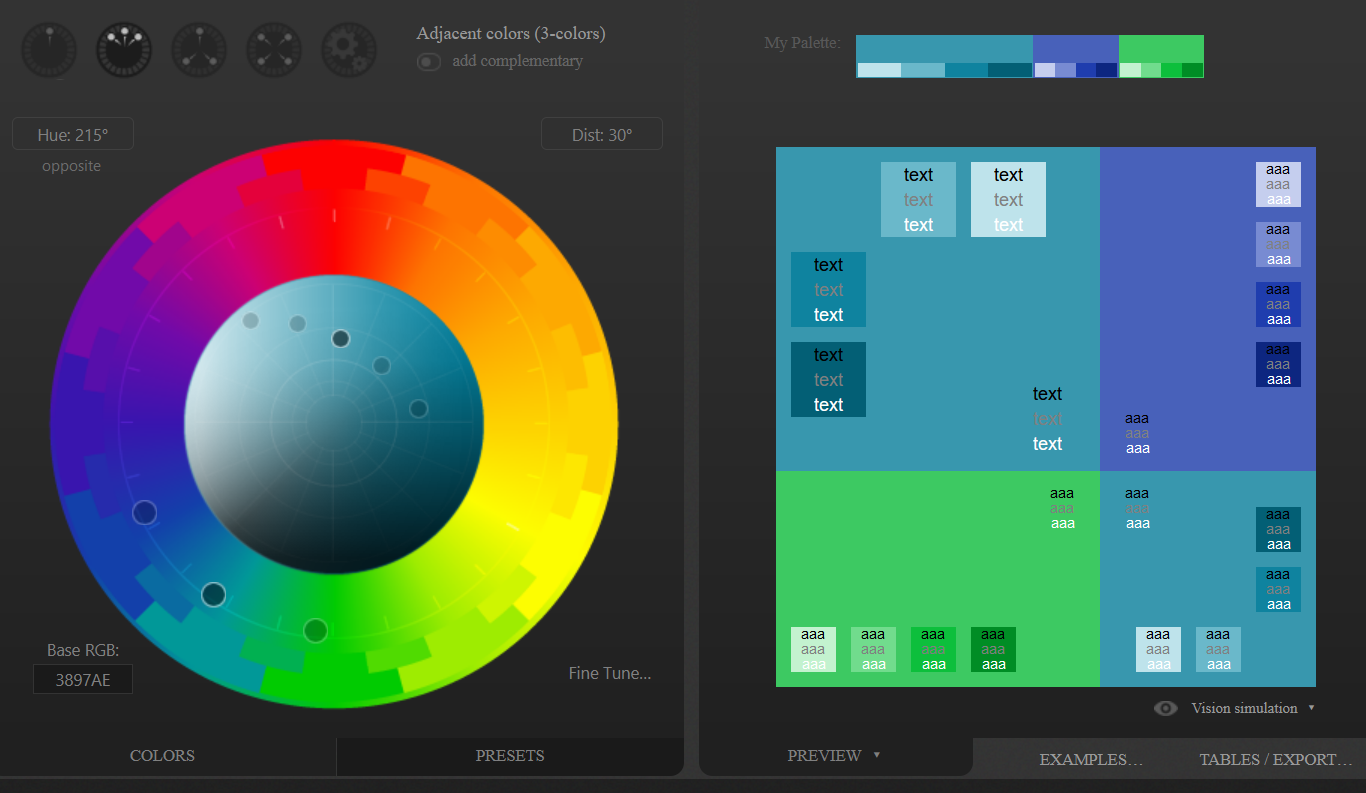
\includegraphics[width=0.8\linewidth]{figures/color-scheme.png}
\caption{Color scheme}
\label{fig:color-scheme}
\end{figure}

\begin{figure}[bh]
    \centering
    \begin{subfigure}[b]{0.4\linewidth}
        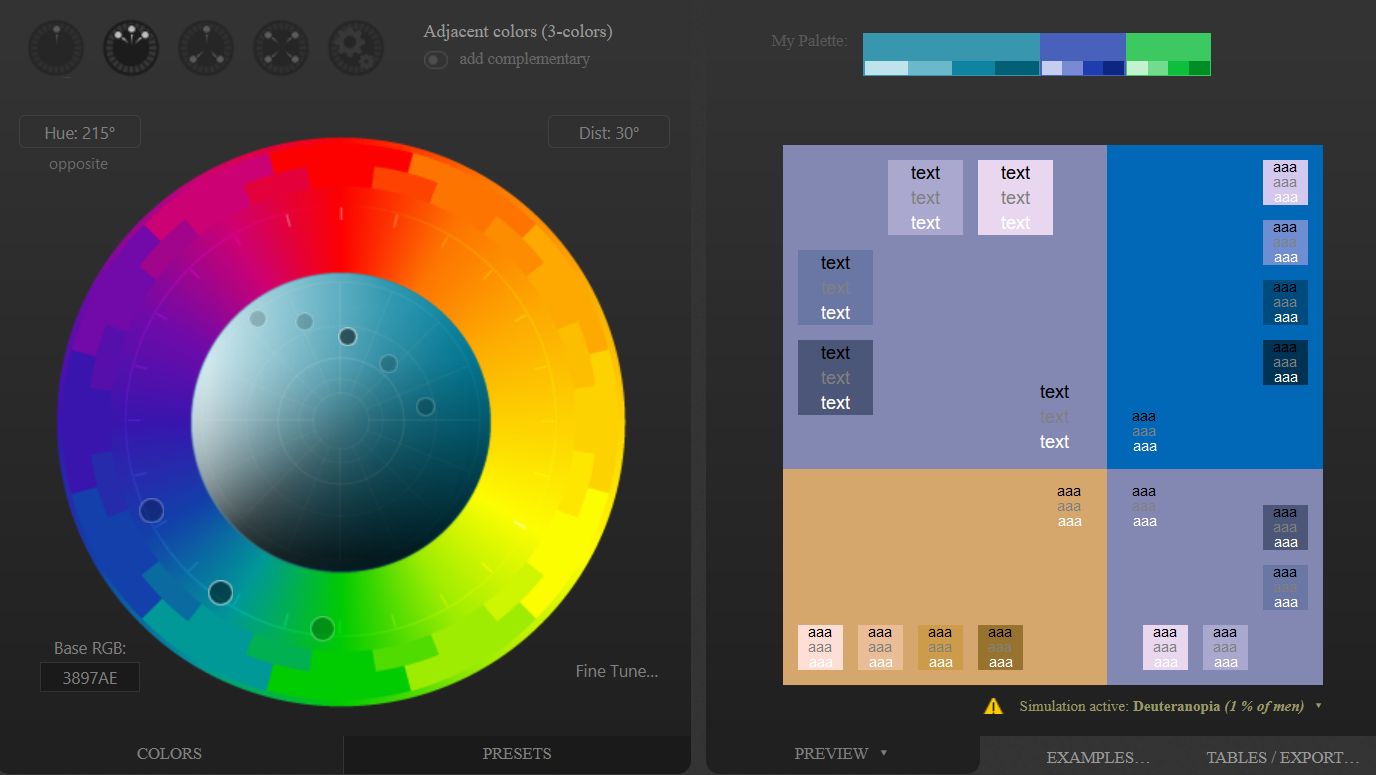
\includegraphics[width=\linewidth]{figures/color-scheme-deuteranopia.png}
        \caption{Deuteranopia}
    \end{subfigure}
    \begin{subfigure}[b]{0.4\linewidth}
        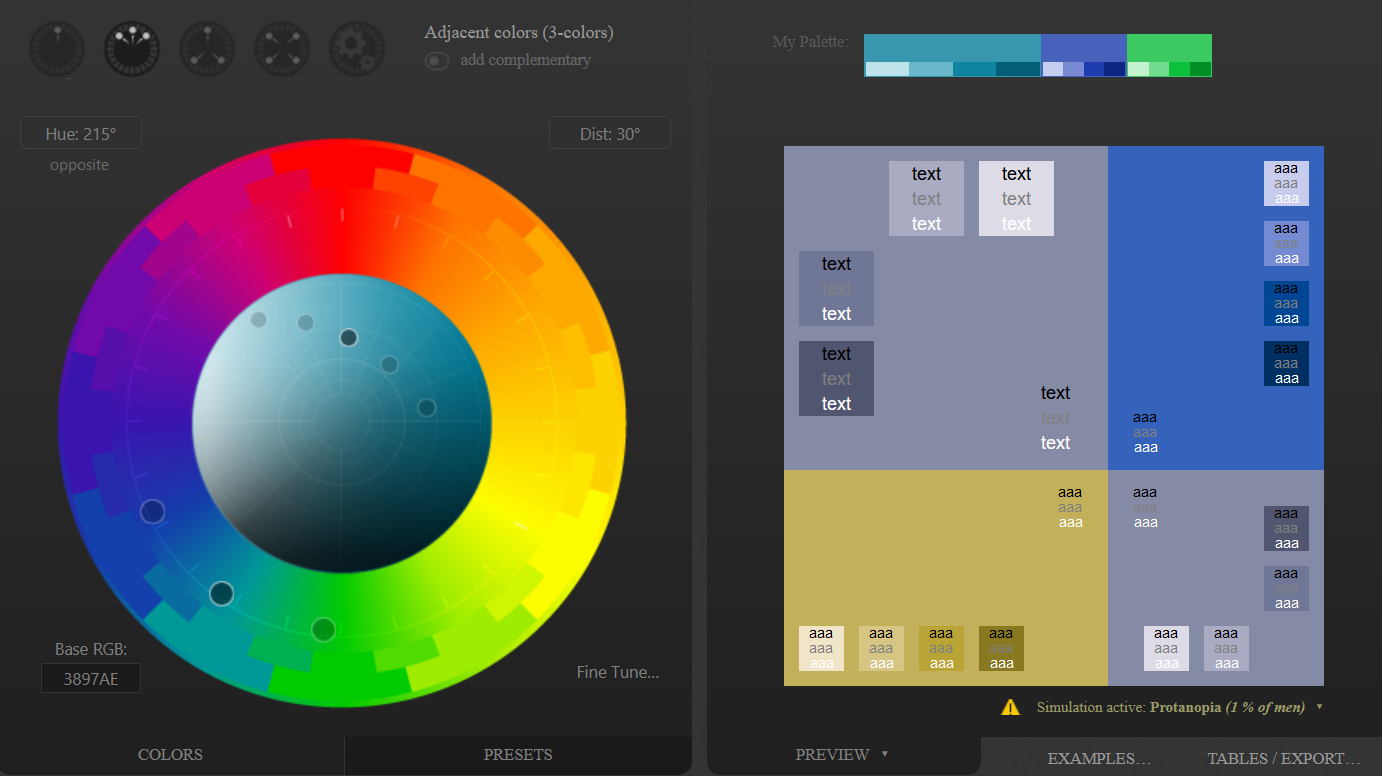
\includegraphics[width=\linewidth]{figures/color-scheme-protanopia.png}
        \caption{Protanopia}
    \end{subfigure}
    \begin{subfigure}[b]{0.4\linewidth}
        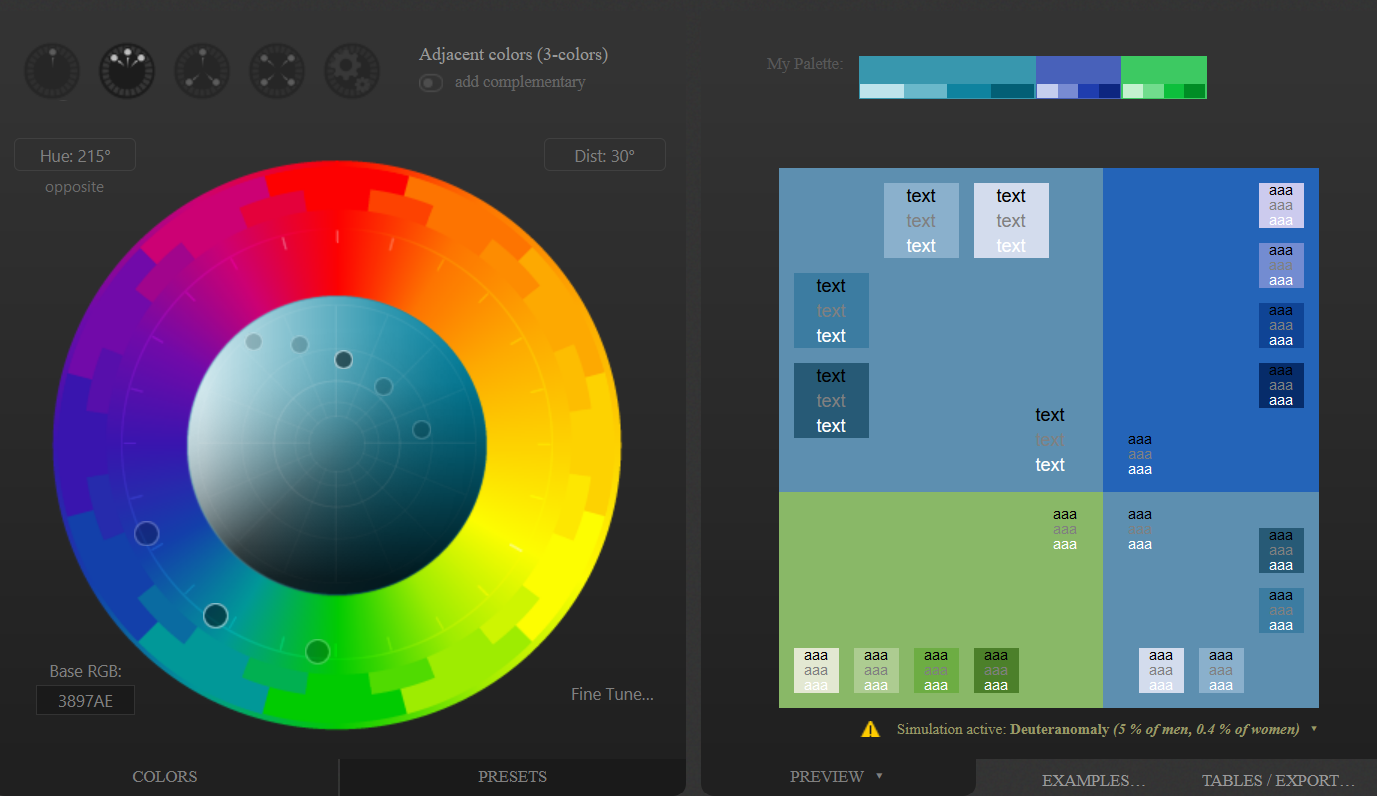
\includegraphics[width=\linewidth]{figures/color-scheme-deuteranomaly.png}
        \caption{Deuteranomaly}
    \end{subfigure}
    \begin{subfigure}[b]{0.4\linewidth}
        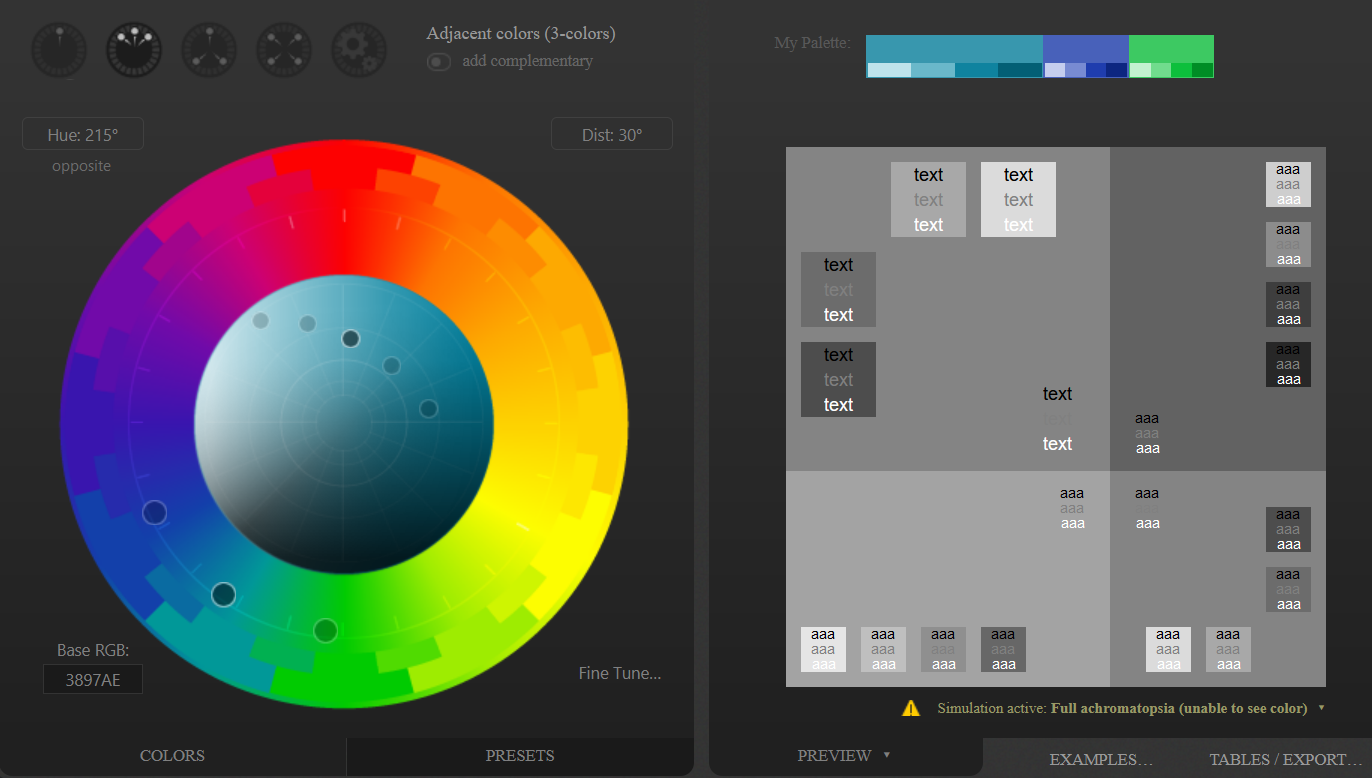
\includegraphics[width=\linewidth]{figures/color-scheme-achromatopsia.png}
        \caption{Achromatopsia}
    \end{subfigure}
\caption{Color Blindness Simulations}
\label{fig:color-scheme-simulations}
\end{figure}

%%%%%%%%%%%%%%%%%%%%%%%%%
%%%%%%%%%%%%%%%%%%%%%%%%%
%%%%%%%%%%%%%%%%%%%%%%%%%
\chapter{Gobbled Lstlistings examples:}\label{results}

\section{Gobbled lstlistings}

\begin{enumerate}
    \item \lstinline[language=bash]{mkdir ~/my-project}

    \item copy whl file in \lstinline{my-project/dist}

    \item Python 3.9 local pyenv

    \begin{lstlisting}[language=bash, title={small Execute in: bash}]
    # @ ~/my-project

    pyenv local 3.9.6
    python -m venv venv
    . venv/scripts/activate    
    \end{lstlisting}

    \item install and set up \lstinline{FLASK_APP}

    \begin{lstlisting}[language=bash, title={small Execute in: bash}]
    # @ ~/my-project (venv)

    pip install package-name-1.0.1-py3-none-any.whl
    export FLASK_APP=package-name
    flask run
    \end{lstlisting}

\end{enumerate}

\section{Design}

We used Paletton. \href{https://paletton.com/#uid=53n0u0kmgAe6fUpfzJrtUwl-jnK}{chosen color scheme}。\footnote{\label{paletton}Paletton color scheme: \href {https://paletton.com/\#uid=53n0u0kmgAe6fUpfzJrtUwl-jnK}{\path{https://paletton.com/#uid=53n0u0kmgAe6fUpfzJrtUwl-jnK}}}

See in fig. \ref{fig:color-palette}.

\begin{figure}[bh]
\centering
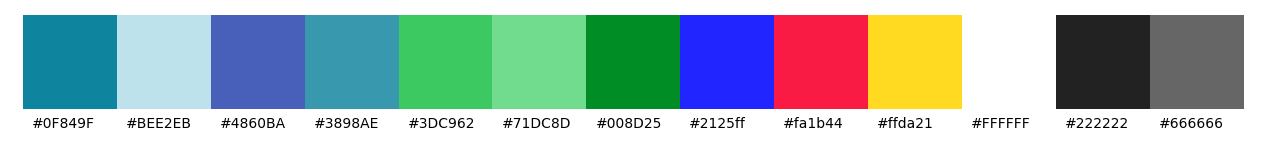
\includegraphics[width=0.6\linewidth]{figures/color-palette.png}
\caption{Color palette}
\label{fig:color-palette}
\end{figure}


%%%%%%%%%%%%%%%%%%%%%%%%%
%%%%%%%%%%%%%%%%%%%%%%%%%
%%%%%%%%%%%%%%%%%%%%%%%%%

\chapter{LaTeX settings}\label{gen_discussion}

\section{XeLaTeX for Japanese}\label{discussion}

\begin{lstlisting}[language={[latex]TeX}, title={small Language: XeLaTeX}]
% !TeX program = XeLaTeX
% !TeX encoding = UTF-8

% For Japanese UTF-8 text in XeLaTeX
\usepackage{xeCJK}
\setCJKmainfont{IPAexMincho}


\usepackage[japanese]{babel} % For Japanese date format
\usepackage{indentfirst} % For Japanese style indentation
\setlength\parindent{11pt}
\end{lstlisting}


For code display:

\begin{lstlisting}[language={[latex]TeX}, title={small Language: XeLaTeX}]
\usepackage[lighttt]{lmodern}
\usepackage{listings} % to display code
\usepackage{lstautogobble} % to indent inside latex without affecting the code, keeping the indent the code has inside
\usepackage{anyfontsize} % for code font size
\usepackage[os=win]{menukeys} % to display keystrokes

% For the color behind the code sections:
\usepackage{xcolor} %custom colours
\definecolor{light-gray}{gray}{0.95} %the shade of grey that stack exchange uses
\definecolor{editorGreen}{rgb}{0, 0.5, 0} % #007C00 -> rgb(0, 124, 0)

% Make a more defined languages for nice colors
\lstdefinelanguage{CSS}{
      keywords={*,html,body,a,h1,h2,h3,h4,h5,h6,h7,h8,h9,p,form,button,label,input,textarea,select,table,th,td,tr,header,footer,and
      },
      morekeywords={[2]{-moz-binding, -moz-border-bottom-colors, -moz-border-left-colors, -moz-border-radius, -moz-border-radius-bottomleft, -moz-border-radius-bottomright, -moz-border-radius-topleft, -moz-border-radius-topright, -moz-border-right-colors, -moz-border-top-colors, -moz-opacity, -moz-outline, -moz-outline-color, -moz-outline-style, -moz-outline-width, -moz-user-focus, -moz-user-input, -moz-user-modify, -moz-user-select, -replace, -set-link-source, -use-link-source, accelerator, align-content, align-items, align-self, animation-delay, animation-direction, animation-duration, animation-fill-mode, animation-iteration-count, animation-name, animation-play-state, animation-timing-function, animation, azimuth, backface-visibility, background, background-attachment, background-clip, background-color, background-image, background-origin, background-position, background-position-x, background-position-y, background-repeat, background-size, behavior, border, border-bottom, border-bottom-color, border-bottom-left-radius, border-bottom-right-radius, border-bottom-style, border-bottom-width, border-collapse, border-color, border-image-outset, border-image-repeat, border-image-slice, border-image-source, border-image-width, border-image, border-left, border-left-color, border-left-style, border-left-width, border-radius, border-right, border-right-color, border-right-style, border-right-width, border-spacing, border-style, border-top, border-top-color, border-top-left-radius, border-top-right-radius, border-top-style, border-top-width, border-width, bottom, box-shadow, box-sizing, caption-side, clear, clip, color, column-count, column-fill, column-gap, column-rule-color, column-rule-style, column-rule-width, column-rule, column-span, column-width, columns, content, counter-increment, counter-reset, cue, cue-after, cue-before, cursor, direction, display, elevation, empty-cells, filter, flex-basis, flex-direction, flex-flow, flex-grow, flex-shrink, flex-wrap, flex, float, font, font-family, font-size, font-size-adjust, font-stretch, font-style, font-variant, font-weight, height, ime-mode, include-source, justify-content, layer-background-color, layer-background-image, layout-flow, layout-grid, layout-grid-char, layout-grid-char-spacing, layout-grid-line, layout-grid-mode, layout-grid-type, left, letter-spacing, line-break, line-height, list-style, list-style-image, list-style-position, list-style-type, margin, margin-bottom, margin-left, margin-right, margin-top, marker-offset, marks, max-height, max-width, min-height, min-width, opacity, order, orphans, outline, outline-color, outline-offset, outline-style, outline-width, overflow, overflow-wrap, overflow-X, overflow-x, overflow-Y, overflow-y, padding, padding-bottom, padding-left, padding-right, padding-top, page, page-break-after, page-break-before, page-break-inside, pause, pause-after, pause-before, perspective-origin, perspective, pitch, pitch-range, play-during, position, quotes, resize, richness, right, ruby-align, ruby-overhang, ruby-position, scrollbar-3d-light-color, scrollbar-arrow-color, scrollbar-base-color, scrollbar-dark-shadow-color, scrollbar-face-color, scrollbar-highlight-color, scrollbar-shadow-color, scrollbar-track-color, size, speak, speak-header, speak-numeral, speak-punctuation, speech-rate, stress, tab-size, table-layout, text-align, text-align-last, text-autospace, text-decoration, text-decoration-color, text-decoration-line, text-decoration-style, text-indent, text-justify, text-kashida-space, text-overflow, text-shadow, text-transform, text-underline-position, top, transform-origin, transform-style, transform, transition-delay, transition-duration, transition-property, transition-timing-function, transition, unicode-bidi, vertical-align, visibility, voice-family, volume, white-space, widows, width, word-break, word-spacing, word-wrap, writing-mode, z-index, zoom
        }}, 
      sensitive=true,
      morecomment=[l]{//},
      morecomment=[s]{/*}{*/},
      morestring=[b]',
      morestring=[b]",
      alsoother={:},
      alsodigit={-},
      tag=[s]
    }
\lstdefinelanguage{HTML5}{
            language=html,
            sensitive=true, 
            alsoletter={<>=-},
            otherkeywords={
            % HTML tags
            <, </, >,
            </a, <a, </a>,
            </abbr, <abbr, </abbr>,
            </address, <address, </address>,
            </area, <area, </area>,
            </area, <area, </area>,
            </article, <article, </article>,
            </aside, <aside, </aside>,
            </audio, <audio, </audio>,
            </audio, <audio, </audio>,
            </b, <b, </b>,
            </base, <base, </base>,
            </bdi, <bdi, </bdi>,
            </bdo, <bdo, </bdo>,
            </blockquote, <blockquote, </blockquote>,
            </body, <body, </body>,
            </br, <br, </br>,
            </button, <button, </button>,
            </canvas, <canvas, </canvas>,
            </caption, <caption, </caption>,
            </cite, <cite, </cite>,
            </code, <code, </code>,
            </col, <col, </col>,
            </colgroup, <colgroup, </colgroup>,
            </data, <data, </data>,
            </datalist, <datalist, </datalist>,
            </dd, <dd, </dd>,
            </del, <del, </del>,
            </details, <details, </details>,
            </dfn, <dfn, </dfn>,
            </div, <div, </div>,
            </dl, <dl, </dl>,
            </dt, <dt, </dt>,
            </em, <em, </em>,
            </embed, <embed, </embed>,
            </fieldset, <fieldset, </fieldset>,
            </figcaption, <figcaption, </figcaption>,
            </figure, <figure, </figure>,
            </footer, <footer, </footer>,
            </form, <form, </form>,
            </h1, <h1, </h1>,
            </h2, <h2, </h2>,
            </h3, <h3, </h3>,
            </h4, <h4, </h4>,
            </h5, <h5, </h5>,
            </h6, <h6, </h6>,
            </head, <head, </head>,
            </header, <header, </header>,
            </hr, <hr, </hr>,
            </html, <html, </html>,
            </i, <i, </i>,
            </iframe, <iframe, </iframe>,
            </img, <img, </img>,
            </input, <input, </input>,
            </ins, <ins, </ins>,
            </kbd, <kbd, </kbd>,
            </keygen, <keygen, </keygen>,
            </label, <label, </label>,
            </legend, <legend, </legend>,
            </li, <li, </li>,
            </link, <link, </link>,
            </main, <main, </main>,
            </map, <map, </map>,
            </mark, <mark, </mark>,
            </math, <math, </math>,
            </menu, <menu, </menu>,
            </menuitem, <menuitem, </menuitem>,
            </meta, <meta, </meta>,
            </meter, <meter, </meter>,
            </nav, <nav, </nav>,
            </noscript, <noscript, </noscript>,
            </object, <object, </object>,
            </ol, <ol, </ol>,
            </optgroup, <optgroup, </optgroup>,
            </option, <option, </option>,
            </output, <output, </output>,
            </p, <p, </p>,
            </param, <param, </param>,
            </pre, <pre, </pre>,
            </progress, <progress, </progress>,
            </q, <q, </q>,
            </rp, <rp, </rp>,
            </rt, <rt, </rt>,
            </ruby, <ruby, </ruby>,
            </s, <s, </s>,
            </samp, <samp, </samp>,
            </script, <script, </script>,
            </section, <section, </section>,
            </select, <select, </select>,
            </small, <small, </small>,
            </source, <source, </source>,
            </span, <span, </span>,
            </strong, <strong, </strong>,
            </style, <style, </style>,
            </summary, <summary, </summary>,
            </sup, <sup, </sup>,
            </svg, <svg, </svg>,
            </table, <table, </table>,
            </tbody, <tbody, </tbody>,
            </td, <td, </td>,
            </template, <template, </template>,
            </textarea, <textarea, </textarea>,
            </tfoot, <tfoot, </tfoot>,
            </th, <th, </th>,
            </thead, <thead, </thead>,
            </time, <time, </time>,
            </title, <title, </title>,
            </tr, <tr, </tr>,
            </track, <track, </track>,
            </u, <u, </u>,
            </ul, <ul, </ul>,
            </var, <var, </var>,
            </video, <video, </video>,
            </wbr, <wbr, </wbr>,
            />, <!
            },  
            morekeywords={[2]{
            % General
            =,
            % HTML attributes
            accept=, accept-charset=, accesskey=, action=, align=, alt=, async=, autocomplete=, autofocus=, autoplay=, autosave=, bgcolor=, border=, buffered=, challenge=, charset=, checked=, cite=, class=, code=, codebase=, color=, cols=, colspan=, content=, contenteditable=, contextmenu=, controls=, coords=, data=, datetime=, default=, defer=, dir=, dirname=, disabled=, download=, draggable=, dropzone=, enctype=, for=, form=, formaction=, headers=, height=, hidden=, high=, href=, hreflang=, http-equiv=, icon=, id=, ismap=, itemprop=, keytype=, kind=, label=, lang=, language=, list=, loop=, low=, manifest=, max=, maxlength=, media=, method=, min=, multiple=, name=, novalidate=, open=, optimum=, pattern=, ping=, placeholder=, poster=, preload=, pubdate=, radiogroup=, readonly=, rel=, required=, reversed=, rows=, rowspan=, sandbox=, scope=, scoped=, seamless=, selected=, shape=, size=, sizes=, span=, spellcheck=, src=, srcdoc=, srclang=, start=, step=, style=, summary=, tabindex=, target=, title=, type=, usemap=, value=, width=, wrap=,
            % CSS properties
            -moz-binding:, -moz-border-bottom-colors:, -moz-border-left-colors:, -moz-border-radius:, -moz-border-radius-bottomleft:, -moz-border-radius-bottomright:, -moz-border-radius-topleft:, -moz-border-radius-topright:, -moz-border-right-colors:, -moz-border-top-colors:, -moz-opacity:, -moz-outline:, -moz-outline-color:, -moz-outline-style:, -moz-outline-width:, -moz-user-focus:, -moz-user-input:, -moz-user-modify:, -moz-user-select:, -replace:, -set-link-source:, -use-link-source:, accelerator:, align-content:, align-items:, align-self:, animation-delay:, animation-direction:, animation-duration:, animation-fill-mode:, animation-iteration-count:, animation-name:, animation-play-state:, animation-timing-function:, animation:, azimuth:, backface-visibility:, background:, background-attachment:, background-clip:, background-color:, background-image:, background-origin:, background-position:, background-position-x:, background-position-y:, background-repeat:, background-size:, behavior:, border:, border-bottom:, border-bottom-color:, border-bottom-left-radius:, border-bottom-right-radius:, border-bottom-style:, border-bottom-width:, border-collapse:, border-color:, border-image-outset:, border-image-repeat:, border-image-slice:, border-image-source:, border-image-width:, border-image:, border-left:, border-left-color:, border-left-style:, border-left-width:, border-radius:, border-right:, border-right-color:, border-right-style:, border-right-width:, border-spacing:, border-style:, border-top:, border-top-color:, border-top-left-radius:, border-top-right-radius:, border-top-style:, border-top-width:, border-width:, bottom:, box-shadow:, box-sizing:, caption-side:, clear:, clip:, color:, column-count:, column-fill:, column-gap:, column-rule-color:, column-rule-style:, column-rule-width:, column-rule:, column-span:, column-width:, columns:, content:, counter-increment:, counter-reset:, cue:, cue-after:, cue-before:, cursor:, direction:, display:, elevation:, empty-cells:, filter:, flex-basis:, flex-direction:, flex-flow:, flex-grow:, flex-shrink:, flex-wrap:, flex:, float:, font:, font-family:, font-size:, font-size-adjust:, font-stretch:, font-style:, font-variant:, font-weight:, height:, ime-mode:, include-source:, justify-content:, layer-background-color:, layer-background-image:, layout-flow:, layout-grid:, layout-grid-char:, layout-grid-char-spacing:, layout-grid-line:, layout-grid-mode:, layout-grid-type:, left:, letter-spacing:, line-break:, line-height:, list-style:, list-style-image:, list-style-position:, list-style-type:, margin:, margin-bottom:, margin-left:, margin-right:, margin-top:, marker-offset:, marks:, max-height:, max-width:, min-height:, min-width:, opacity:, order:, orphans:, outline:, outline-color:, outline-offset:, outline-style:, outline-width:, overflow:, overflow-wrap:, overflow-X:, overflow-x:, overflow-Y:, overflow-y:, padding:, padding-bottom:, padding-left:, padding-right:, padding-top:, page:, page-break-after:, page-break-before:, page-break-inside:, pause:, pause-after:, pause-before:, perspective-origin:, perspective:, pitch:, pitch-range:, play-during:, position:, quotes:, resize:, richness:, right:, ruby-align:, ruby-overhang:, ruby-position:, scrollbar-3d-light-color:, scrollbar-arrow-color:, scrollbar-base-color:, scrollbar-dark-shadow-color:, scrollbar-face-color:, scrollbar-highlight-color:, scrollbar-shadow-color:, scrollbar-track-color:, size:, speak:, speak-header:, speak-numeral:, speak-punctuation:, speech-rate:, stress:, tab-size:, table-layout:, text-align:, text-align-last:, text-autospace:, text-decoration:, text-decoration-color:, text-decoration-line:, text-decoration-style:, text-indent:, text-justify:, text-kashida-space:, text-overflow:, text-shadow:, text-transform:, text-underline-position:, top:, transform-origin:, transform-style:, transform:, transition-delay:, transition-duration:, transition-property:, transition-timing-function:, transition:, unicode-bidi:, vertical-align:, visibility:, voice-family:, volume:, white-space:, widows:, width:, word-break:, word-spacing:, word-wrap:, writing-mode:, z-index:, zoom:
            }},  
            morecomment=[s]{<!--}{-->},
            tag=[s]
    }

% Set up the code display lst options
\lstset{
    % for the code font and size:
    % basicstyle=\ttfamily\small,
    basicstyle=\ttfamily\fontsize{10}{12}\selectfont,
    % to avoid spaces showing as brackets in strings
    showstringspaces=false,
    % for straight quotes in code
    upquote=true, 
    % for the middle tildes in the code
    literate={~}{{\fontfamily{ptm}\selectfont \textasciitilde}}1,
    % for the line break in long texts
    breaklines=true,
    postbreak=\mbox{\textcolor{red}{$\hookrightarrow$}\space}, 
    % for the keyword colors in the code
    keywordstyle=\color{blue}\bfseries\ttfamily,
    stringstyle=\color{purple},
    commentstyle=\color{darkgray}\ttfamily,
    keywordstyle={[2]{\color{editorGreen}\bfseries\ttfamily}},
    autogobble=true % to ignore latex indents but keep code indent
}

% unnecessary in XeLaTeX
% % For this specific document with lots of degree signs inside listings
% \lstset{
%     literate={°}{\textdegree}1
% }

% for straight double quotes in code
\usepackage[T1]{fontenc}

% frame set up
\usepackage[framemethod=TikZ]{mdframed} %nice frames
\mdfsetup{
    backgroundcolor=light-gray,
    roundcorner=7pt,
    leftmargin=1,
    rightmargin=1,
    innerleftmargin=1em,
    innertopmargin=0.5em,
    innerbottommargin=0,
    outerlinewidth=1,
    linecolor=light-gray,
    } 

% Make it affect all lstlistings
\BeforeBeginEnvironment{lstlisting}{\begin{mdframed}\vskip-.5\baselineskip}
\AfterEndEnvironment{lstlisting}{\end{mdframed}}

% Make colored box around inline code
\usepackage{realboxes}
\usepackage{xpatch}

\makeatletter
\xpretocmd\lstinline{\Colorbox{light-gray}\bgroup\appto\lst@DeInit{\egroup}}{}{}
\makeatother
\end{lstlisting}

Download \href{}{\lstinline{lststyle-css.sty}} and \href{}{\lstinline{lststyle-html5.sty}} for the colored keywords in CSS and HTML.


%%%%%%%%%%%%%%%%%%%%%%%%%
%%%%%%%%%%%%%%%%%%%%%%%%%
%%%%%%%%%%%%%%%%%%%%%%%%%

\clearpage

\printbibliography[heading=bibintoc]

% \end{CJK}
%unnecessary in XeLaTeX

\end{document}